\subsubsection{Manuelle Auswertung der Schwebung}
Eine Manuelle Auswertung des Schwebungsinterferogramms wird trotz Schwierigkeiten so weit wie m�glich durchgef�hrt.
Die beiden Wellenl�ngen $\lambda_-$ und $\lambda_+$ werden wie zuvor bestimmt (vgl. \ref{sec:chopper}). F�r $\lambda_+$ ein Werte von 275,6(3) $\mu$m bestimmt, indem �ber eine 1/2-Periode gez�hlt wurde. F�r $\lambda_-$ wurde ein Wert von 3,15(3) $\mu$m bestimmt (vgl. Tabelle \ref{tab:wellenlaengen_messung}). 

\begin{table}[H]
\centering
\caption{Bestimmte Wellenl�ngen $\lambda_{+,-}$, vlg. Abbildung ??}
\label{tab:wellenlaengen_messung}
\begin{tabular}{|c|c|c|c|c|c|}
\hline  & n & s$_1$ /mm & s$_2$ / mm & $\Delta$s / mm & $\lambda$ / $\mu$m \\ 
\hline $\lambda_{+}$ & 1/2 & 4.7911(2) & 4.6535(2) & 0.1376(3) & 275.6(3) \\ 
\hline $\lambda_{-}$ & 4 & 4.7911(2) & 4.9177(2) & 0.1266(3) & 3.15(3) \\ 
\hline 
\end{tabular} 
\end{table}

Mit den Wellenl�ngen $\lambda_{+,-}$ k�nnen mit Gleichung \ref{eqn:lambda+} und \ref{eqn:lambda-} die Wellenl�ngen des Schmalbandfilters und des Lasers bestimmt werden. Alle bestimmten Wellenl�ngen sind in Tabelle \ref{tab:wellenlaengen} eingetragen.

\begin{table}[H]
\centering
\caption{Bestimmte Wellenl�ngen $\lambda_{Laser,Muffelofen,+,-}$}
\label{tab:wellenlaengen}
\begin{tabular}{|c|c|}
\hline $\lambda_{Laser}$ & \SI{3,11(4)}{$\mu$m} \\ 
\hline $\lambda_{SBF}$ & \SI{3.18(4)}{$\mu$m} \\ 
\hline $\lambda_{+}$ & \SI{275,6(3)}{$\mu$m} \\ 
\hline $\lambda_{-}$ & \SI{3,15(3)}{$\mu$m} \\ 
\hline 
\end{tabular} 
\end{table}

Die Parameter $2\pi b_{Laser}$ und $2\pi b_{SBF}$ werden wie in Abschnitt \ref{sec:filter} bestimmt, der Parameter $a$ wird �bernommen. Es ergeben sich die Werte in Tabelle \ref{tab:parameter_2}.

\begin{table}[H]
\centering
\caption{Parameter f�r die spektrale Verteilung}
\label{tab:parameter_2}
\begin{tabular}{|c|c|}
\hline $a$ & 0,0129(1) mm \\ 
\hline $2\pi b_{Laser}$ & \SI{1,863(5)}{$\mu$m} \\
\hline $2\pi b_{SBF}$ & \SI{2,159(37)}{$\mu$m} \\
\hline 
\end{tabular} 
\end{table}

Mit den Werten aus Tabelle \ref{tab:parameter_2} ergibt sich die spektrale Verteilung in Abbildung \ref{fig:spektrum_schwebung}.

\begin{figure}[H]
\centering
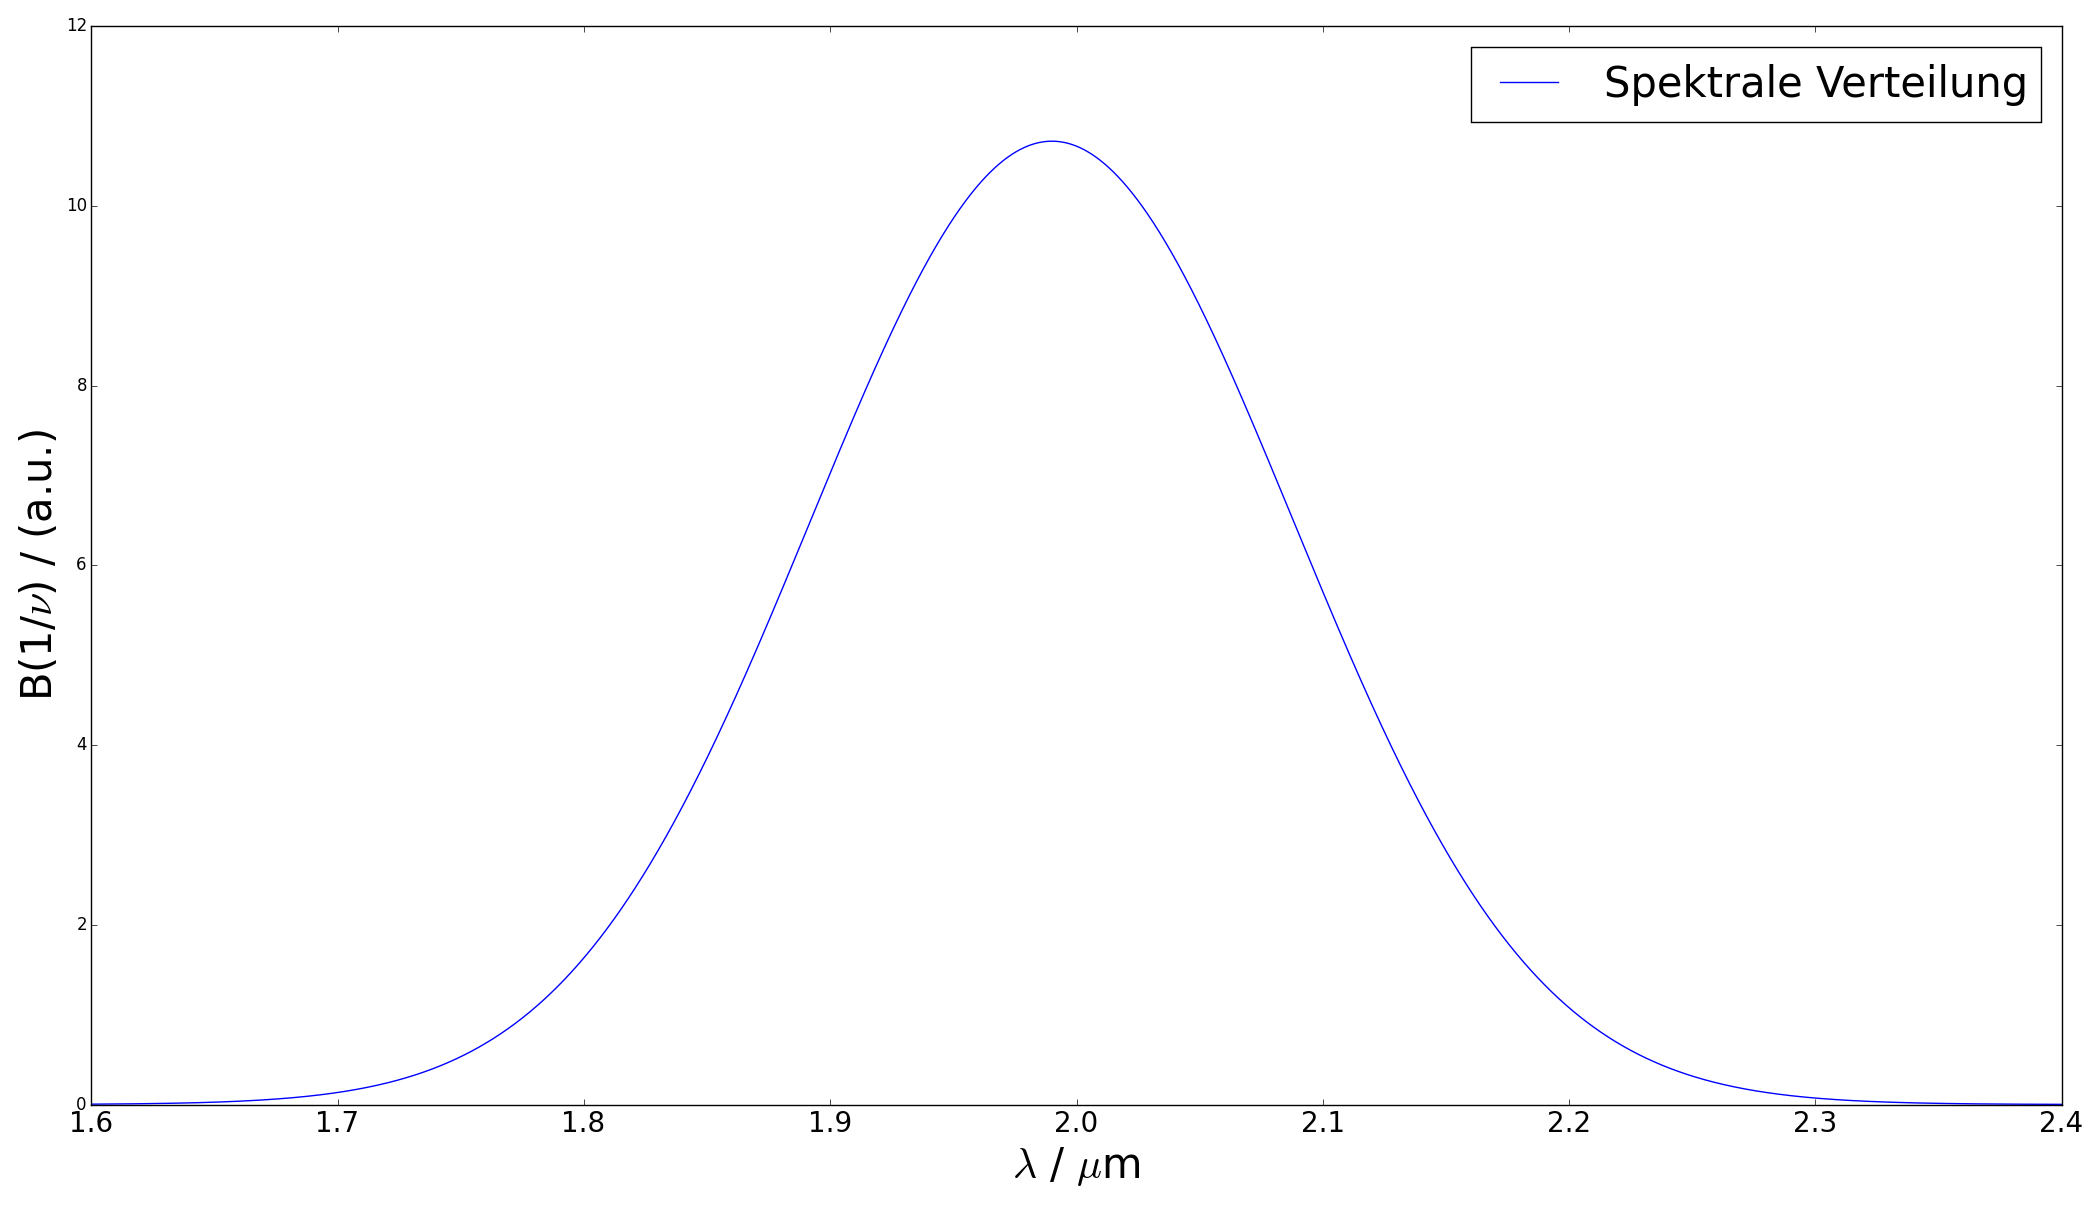
\includegraphics[scale = 0.33]{verteilung_schwebung.png}
\caption{Spektrale Verteilung der Schwebung}
\label{fig:spektrum_schwebung}
\end{figure}